\documentclass[13pt]{beamer}
\mode<beamer>{%
  \usetheme[]{CambridgeUS}}
\usepackage{lmodern, amssymb,amsmath, graphicx, hyperref}
\usepackage[normalem]{ulem}
\usepackage{csquotes}
\graphicspath{{gh-pages/Figs/}}

 \title{Unequal Representation:} 
 \subtitle{Constituency Service in Today's Congress}
    \author[Judge-Lord, Grimmer, Powell]{Eleanor Neff Powell \\ Booth Fowler Associate Professor \\ University of Wisconsin-Madison}
    \date[\today]{Joint with Devin Judge-Lord\thanks{Ph.D. Candidate, University of Wisconsin-Madison} and Justin Grimmer\thanks{Professor, Stanford University} \\ \bigskip \today}
\begin{document}
\begin{frame}
\maketitle
\end{frame}

% Hi, My name is Devin Judge-Lord
% I am presenting work with coauthors Justin Grimmer and Ellie Powell based on a very large new database of letters and emails written by members of Congress to federal agencies. We have spent the past 2 years collecting and coding these data, and I am excited to share the very first results from this project. 

% We started with a common intuition that Members of Congress have limited time and attention to divide among, for example, constituency work and policy work. We have come to question the value of this intuition for explaining  at least this aspect of legislator behavior.
% We did not find a tradeoff between being attentive to constituents and influential in washingon; instead, by our measure, some legislators are both and some are neither.

% I am going to introduce our data and show that, in fact, the same members who do more policy work also do more constituency service and that both seem to be connected to institutional power. 

% But first, I want to talk a little bit about our definitions and intuitions about constituency service.

% From where did our, possibly incorrect intuition arise? [SLIDE]

%%%%%%%%%%%%%%%%%%%%%%%%%%%%%%
\begin{frame} 
\frametitle{Rethinking Representation in Congress}
\Large
How do we measure quality of representation?

\begin{itemize}
\item \textbf{Ideological fit}
\item \textbf{Legislative Effectiveness}
\item \textbf{Constituency Service} \alert{$\leftarrow$ Our New Approach}
\end{itemize}
\end{frame}
%%%%%%%%%%%%%%%%%%%%%%%%%%%%%
\begin{frame}
\frametitle{What is Constituency Service?}
\begin{center}
\Large
\textit{``help to individuals, groups, and localities \\ in coping with the federal government.''}\\  -- Fenno (1978)
\end{center}
\end{frame}

%%%%%%%%%%%%%%%%%%%%%%%%%%%%%
\begin{frame}

\begin{center}
\Large
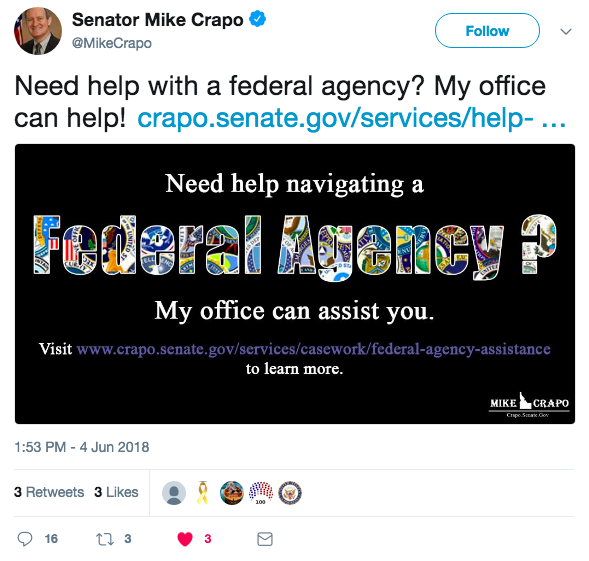
\includegraphics[width = \textwidth]{help}
\end{center}
\end{frame}


%%%%%%%%%%%%%%%%%%%%%%%
\begin{frame}
\Large
\frametitle{Classic Examples:} 
\begin{itemize}
\item Help with an immigration case
\item Help with social security benefits
\item Help with veteran's benefits
\pause 
\bigskip
\item Non-Ideological
\item Helping Constituents Solve Problems
\end{itemize}
\end{frame}
%%%%%%%%%%%%%%%%%%%%%%%%%%%%%%%%
\begin{frame}
\frametitle{What do we know about constituency service?}
\Large
\begin{itemize}
\item Congressional scholars *think* they know a lot.
\item It contributes to a member's personal vote (Fiorina).
\item \alert{BUT ... } we've never had any hard data on it.
\item Behind the scenes:
\begin{itemize}
\item Difficult for academics to study 
\item Difficult for voters to monitor.
\end{itemize}
\end{itemize}
\end{frame}
%%%%%%%%%%%%%%%%%%%%%%%%%%%%%%%%

%%%%%%%%%%%%%%%%%%%%%%%%%%%%%%
\begin{frame}
\frametitle{How Constituency Service Works}
\Large
Step 1: Constituent writes/calls Legislator
\bigskip

Step 2: Legislator writes/calls Agency  

\bigskip
Step 3: Legislator writes to Constituent



\end{frame}
%%%%%%%%%%%%%%%%%%%%%%%%%%%%%%%
%%%%%%%%%%%%%%%%%%%%%%%%%%%%%%
\begin{frame}
\frametitle{How Constituency Service Works}
\Large
Step 1: Constituent writes/calls Legislator
\bigskip

Step 2: Legislator writes/calls Agency \hspace{1cm} \textbf{\alert{$\longleftarrow$}}

\bigskip
Step 3: Legislator writes to Constituent



\end{frame}
%%%%%%%%%%%%%%%%%%%%%%%%%%%%%%%
%%%%%%%%%%%%%%%%%%%%%%%%%%%%%%
\begin{frame}
\frametitle{How Constituency Service Works}
\Large
Step 1: Constituent writes/calls Legislator
\bigskip

\sout{Step 2: Legislator writes/calls Agency }

\bigskip
Step 3: Legislator writes to Constituent



\end{frame}
%%%%%%%%%%%%%%%%%%%%%%%%%%%%%%%


\begin{frame}
\frametitle{Creating the first systematic constituency service data}
\Large
\begin{itemize}
\item Requests that members of Congress made directly to parts of the federal bureaucracy.
\begin{itemize}
\item Letters, emails, phone calls
\end{itemize}
\item Obtained through FOIA requests to all agencies.
\item Usually obtained a summary of the request.
\item Somtimes obtained the written request itself.
\end{itemize}
\end{frame}

%%%%%%%%%%%%%%%%%%%%%%%%%%%%%%%%%%%%%%%%%
\begin{frame}
\frametitle{Note: Prior Studies Using FOIA Approach}
\begin{itemize}
 \item Represent constituents' policy demands despite party pressure (Ritchie 2017) 
% % Ritchie finds that when legislators face cross-pressures on policy issues, they directly engage the bureaucracy in order to still represent constituents even though party politics keep them from doing so legislatively. 
 \item Constituents and institutional position, not ideology, drive policy oversight (Lowande 2018) 
% % Lowande, also focusing on policy, finds that partisan disagreement with the executive branch does not drive oversight.
 \item Descriptive $\rightarrow$ substantive (Lowande, Ritchie, Lauterbach, 2018)
% % Lowande, Ritchie, and Lauterbach show that legislators make more requests on behalf of constituents with whom they share marked identities
 \item Bureaucrats have reasons to comply
   \begin{itemize} 
     \item And they do (Ritchie and You n.d.). 
    \item Though not always (Mills and Kalaf-Hughes 2015))
\end{itemize}
\end{itemize}

\end{frame}
%%%%%%%%%%%%%%%%%%%%%%%%%%%%%%%%
%%%%%%%%%%%%%%%%%%%%%%%%%%%%%%%
\begin{frame}
\frametitle{Limitation of Prior Studies Using FOIA Approach}

\LARGE

\begin{itemize}
\item Based on a small number of agencies.
\end{itemize}

\end{frame}
%%%%%%%%%%%%%%%%%%%%%%%%%%%%%%%%
\begin{frame}
\frametitle{Our Correspondence Data}
\Large
\begin{itemize}
\item 250+ FOIA requests to 233 federal agencies (a census)
\item Data Coverage: 2007-2018
\item We began placing these requests 2.5 years ago.
\item 150,000+ legislator requests (and counting)
\end{itemize}
% to collect these data we have filed over 250 freedom of information act requests, and I continue to follow up on new leads. Some agencies said it would take two years, and they were not exaggerating. I have ongoing email threads and notes from phone calls with hundreds of different FOIA officers. 
 
% Our aim a census of all correspondence 
% our data are incomplete but nevertheless cover a wide swath of the federal government, to the point where we can start to infer a total volume. 

% In our analysis below our DV is the number of letters each legislator writes PER AGENCY, and because we view the federal government as many component agencies, these estimates can probably be multiplied by 100-200 agencies to get the government-wide effect. 
\end{frame}


\begin{frame}
\frametitle{Our Correspondence Data}
\scriptsize
% response table
\begin{table}[!htbp] \centering 
  % \caption{} 
  \label{} 
\begin{tabular}{@{\extracolsep{5pt}} lcccc} 
 & FOIAed  & Records & Coded & N \\ 
 &Components&Received&&\\
\hline \\[-1.8ex] 
Department of Agriculture & 29 & 29 & 11 & 1957 \\ 
Department of Commerce & 18 & 18 & 10 & 6875 \\ 
Department of Defense & 49 & 10 & 7 & 5479 \\ 
Department of Education & 1 & 1 & 1 & 3868 \\ 
Department of Energy & 8 & 2 & 1 & 1269 \\ 
Department of Health and Human Services & 15 & 7 & 5 & 6199 \\ 
Department of Homeland Security & 6 & 5 & 5 & 26435 \\ 
Department of Housing \& Urban Dev. & 2 & 0 & 0 & 0 \\ 
Department of Justice & 11 & 1 & 1 & 903 \\ 
Department of Labor & 24 & 9 & 6 & 22936 \\ 
Department of State & 1 & 0 & 0 & 0 \\ 
Department of the Interior & 10 & 6 & 5 & 5171 \\ 
Department of the Treasury & 8 & 5 & 4 & 11143 \\ 
Department of Transportation & 10 & 6 & 6 & 18482 \\ 
Department of Veterans Affairs & 3 & 0 & 0 & 0 \\ 
\hline \\[-1.8ex] 
Independent Agencies & 38 & 21 & 18 & 46182 \\ 
\hline \\[-1.8ex] 
Total & 233 & 120 & 80 & 156899 \\ 
\hline \\[-1.8ex] 
\end{tabular} 
\end{table} 

\end{frame}
%%%%%%%%%%%%%%%%%%%%%%%%%%%%%%%%
\begin{frame}
\frametitle{Format of Data We Received}
\begin{itemize}
\item Digital Spreadsheets
\item PDFs
\item Scans of Handwritten Documents
\item CD-ROMS
\item Photocopies
\end{itemize}
\end{frame}
%%%%%%%%%%%%%%%%%%%%%%%%%%%%%%%%

% To study who does constituency service and when they do it, we assemble a new dataset of requests--letters, emails, phone calls that members of Congress made directly to parts of the federal bureaucracy.




\begin{frame}
\frametitle{Correspondence Data}
Environmental Protection Agency
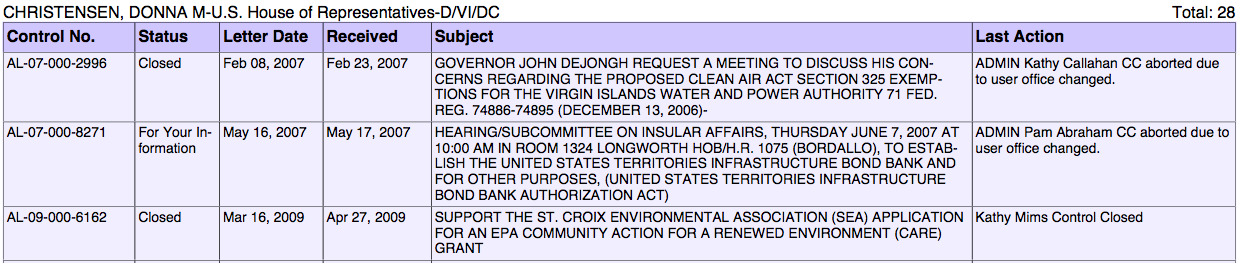
\includegraphics[width = \textwidth]{EPA}
% rich and informative summaries like those kept by the EPA. Here, Rep Donna writes about a regulatory exemption for a power plant, to alert EPA to a hearing, and in support of a nonprofit grant application.
\end{frame}


% To give you a sense of the range of responses. Some agencies provided letters themselves,

%{SLIDE}

% others provided logs, which range widely in the amount of information they record. 
% from, at the worst, handwritten logs with obscure acronyms to indicate the topic, as in this log from ICE
\begin{frame}
\frametitle{Correspondence Data}
Department of Homeland Security Immigration and Customs Enforcement (ICE)
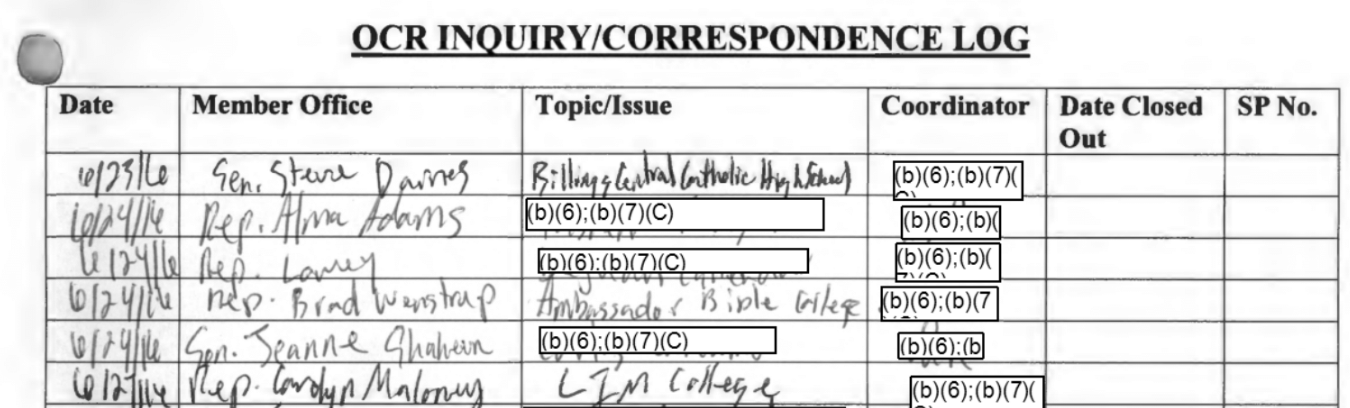
\includegraphics[width = \textwidth]{ICE}
\end{frame}

% Or, in contrast [SLIDE]
\begin{frame}
\frametitle{Correspondence Data}
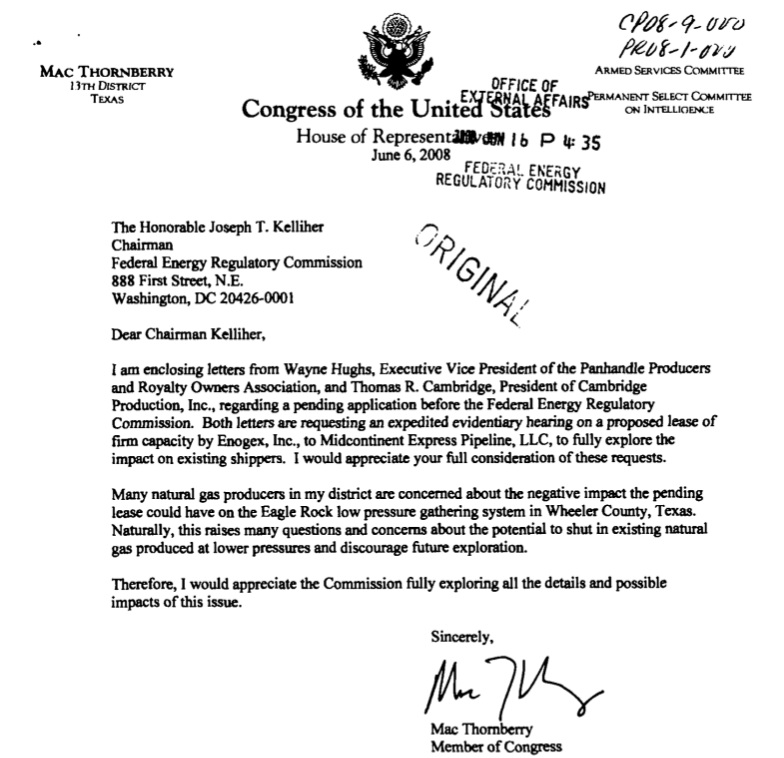
\includegraphics[width = \textwidth]{FERC}
% For example, here Rep. Thornberry, chair of armed services committee is writing to Federal Energy Regulatory Commission on behalf of two companies in his district, asking for extra scrutiny on a another company's permit application. 

% We have several thousand such letters written to this agency, which we use optical content recognition to extract the text. If they do not have metadata like the sender's name and date, we extract it from the text of the letter or discription of the letter.
\end{frame}



\begin{frame}
\frametitle{Agency Character: CIA $\#$OnBrand}
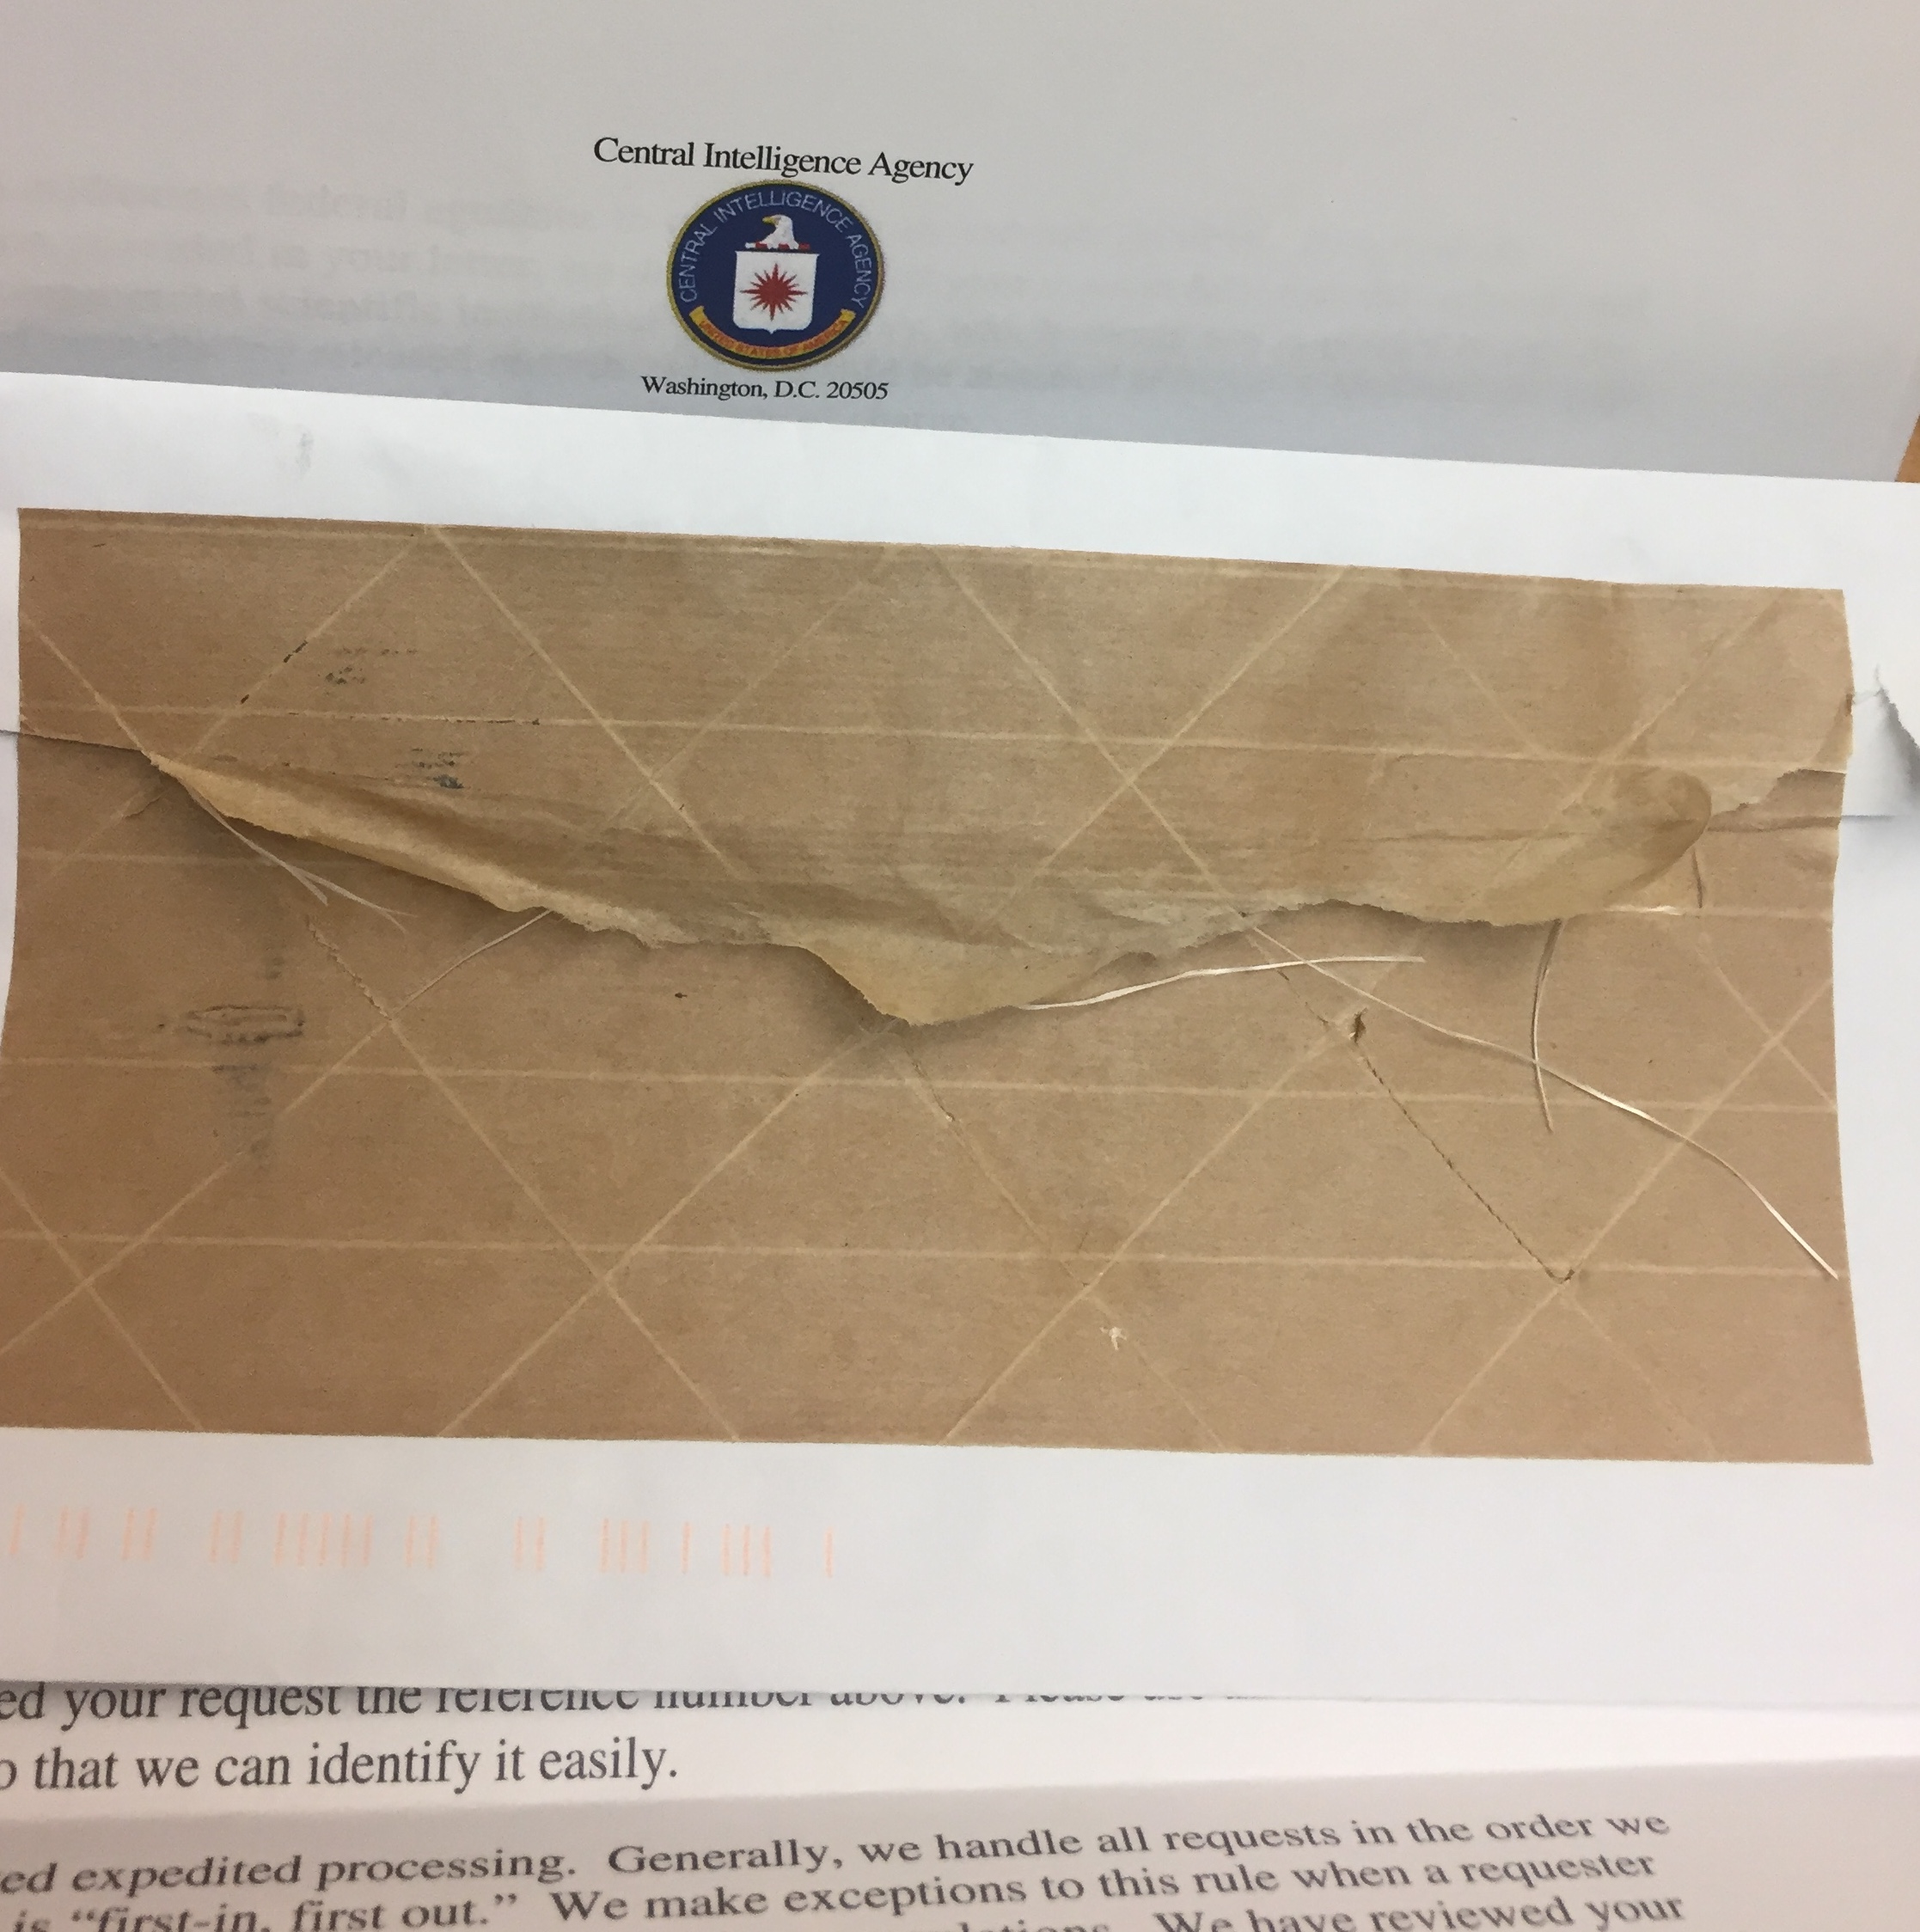
\includegraphics[width = \textwidth]{CIACorrespondence}
\end{frame}

% [SLIDE]





% We trained undergraduate and graduate RAs to code these letters according to a codebook. This analysis relies on our most high-level coding: the type of letter:

% [SLIDE] So far we have over 90,000 coded. 

% And here is the distribution across types. 
% THIS IS TOTAL NUMBER OF LETTERS, EMAILS, ETC, by TYPE 
% By far individual consituent service is the most common reason for a legislator to contacgt an agency.

\begin{frame}
\frametitle{Distribution} 
\begin{figure}[hbt!]
\centering
\caption{Distribution Across Types of Congressional Requests 2007-2017}
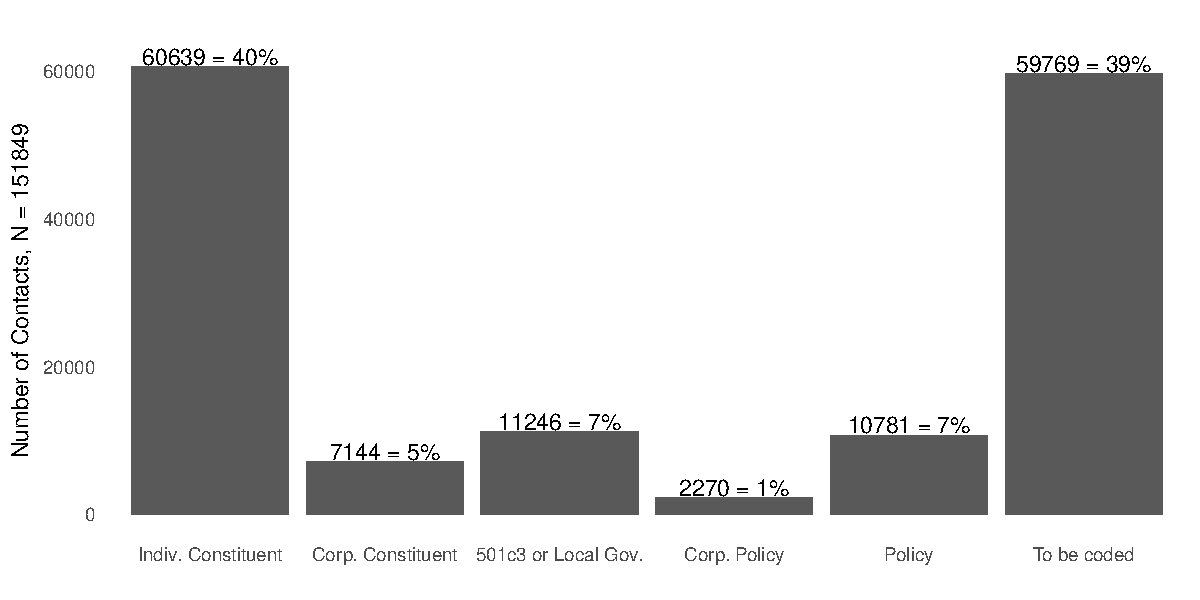
\includegraphics[width = \linewidth]{data_by_type.pdf}
\end{figure}
\end{frame}




% Surely, some of this rhetoric is accusing legislators of not VOTING how their constituents would want. But of course, representation goes beyoned floor votes.
% Indeed there are far more intimate forms of representation that are less constrained by parties and by chamber procedure.

% Possibly the most common act of representation is helping constituents deal with the bureaucracy. 

% %[slide]
% 
% 
% \begin{frame}
% \frametitle{}
% \only<1>{
\includegraphics[width = \textwidth]{tweet}}
% \only<2>{
\includegraphics[width = \textwidth]{durbin-position}}
% \end{frame}
% %This has been true since legislators helped constituents get pensions after the revolutionary war and especially with the rise of the administrative state. Federal agencies now shape nearly every aspect of our lives: 
% 
% % Thus, we focus on the requests legislators and their staff send to federal agencies.
% 
% % [SLIDE} 
% 
% \section{Why legislators lobby the bureaucracy?}
% \begin{frame}
% \frametitle{ What do we know?}
% \Large 
% Exciting new research: \pause
% % This aspect of representation has only begun to be studied but has already yielded some really exciting findings: 
% % Data on legislator requests to agencies has opened a whole new way to study representation: 
% % So what do we know about why legislators lobby the bureaucracy? 
% 
% % [SLIDE]
% \begin{itemize}
% \item Represent constituents' policy demands despite party pressure (Ritchie, 2017) 
% % Ritchie finds that when legislators face cross-pressures on policy issues, they directly engage the bureaucracy in order to still represent constituents even though party politics keep them from doing so legislatively. 
% \item Constituents and institutional position, not ideology, drive policy oversight (Lowande, 2018) 
% % Lowande, also focusing on policy, finds that partisan disagreement with the executive branch does not drive oversight.
% \item Descriptive $\rightarrow$ substantive (Lowande, Ritchie, Lauterbach, 2018)
% % Lowande, Ritchie, and Lauterbach show that legislators make more requests on behalf of constituents with whom they share marked identities
% \item Bureaucrats have reasons to comply
%   \begin{itemize} 
%     {\large \item And they do (Ritchie and You, n.d.). }
%     {\large \item Though not always (Mills and Kalaf-Hughes, 2015))}
%   \end{itemize}
% \end{itemize}
% \end{frame}
% % Recent work by Ritchie and You and Mills and Kalaf-Hughes has begun to investigate whether legislator requests matter and find that they do.
% 
% 
% % Building on this work, we focus squarely on constituency service [SLIDE]



% But there is large variance across members. Gini coefficients in letter writing are much higher than, campaign spending, for example, approximately comparable to income inequality in the US and Mexico. 
% THIS IS THE AVERAGE LETTERS PER YEAR BY PERCENTILE IN EACH CHAMBER
% Schumer, Specter, Gillabrand, Warren, Grassley, average 3 to 5 times as many requests per year as the median senator
%%%%%%%%%%%%%%%%%%%%%%%%%%%%%%%%%%%%%%%%%%%%%
\begin{frame}
\Large
\begin{center}
Do constituents in different districts receive comparable representation?
\end{center}
\end{frame}

%%%%%%%%%%%%%%%%%%%%%%%%%%%%%%%%%%%%%%%%%%%%%
\begin{frame}
\frametitle{Highly Unequal Rates: Variation in Who Contacts Agencies} 
\begin{figure}
\centering

\includegraphics[width = \textwidth]{percentiles-1}
\end{figure}
\end{frame}
% [NOTE: Ellie and Justin, I considered changing this to a histogram, but upon reflection, it seems that mean per member per year is a more interesting axis than number per percentile (as a histogram with bin = 100 would show). As a pattern, they look the same. However, I would be interested to hear any counterarguments.]

\begin{frame}
\frametitle{Highly Unequal Rates} 
\Large
\begin{itemize}
\item High levels of inequality
\bigskip
\item Gini-Coefficient for House $\sim$ US Income Inequality 
\end{itemize}
\end{frame}


% Senators with larger state populations, and thus more demand for constituency service do write more letters, but there are significant outliers. 
%%%%%%%%%%%%%%%%%%%%%%%%%%%%%%%%%%%%%%%%%%
\begin{frame}
\Large
\begin{center}
Are these differences driven by constituent demand?
\end{center}

\end{frame}
%%%%%%%%%%%%%%%%%%%%%%%%%%%%%%%%%%%%%%%%%%
\begin{frame}
\frametitle{Constituency Demand} 
\begin{figure}
\centering
\caption{Senators from larger states do more constituency  service, but ...}

\includegraphics[width = 4in]{population-1}
\end{figure}
\end{frame}


%[SLIDE]


\begin{frame}
\centering
\huge
So why do some legislators do more constituency service than others?
\end{frame}

%%%%%%%%%%%%%%%%%%%%%%%%%%%%%%%

\begin{frame} 
\frametitle{Institutional Explanations: A constituent-policy trade-off?}
\huge 
\begin{itemize}
\item ``Potomac fever'' (Fenno, 1978) \pause
% it emerges from scholarship. Fenno talks about Potomac Feaver--the idea that the deeper a legislator gets into Washington policymaking, the less time they had for their district constituents--thus COMPETING goals of good policy and influence in washington and reelectoin.
\item ``Insiders'' who have lost touch \pause
% we also see it in the popular press and campaign rhetoric contrasting Washington insiders and policy wonks with outsiders who are more in touch with real americans. 
\item \#DrainTheSwamp
% It is evoked in rallying cries to `drain the swamp' of a policy-focused elite who no longer serve their constituents.
\end{itemize}
\end{frame}


% So what is it about some legislators compared to others that we see such dramatic variance in lobbying the bureaucracy? 
% Our original intuition was that some members had reason to prioritize constitute service and others had reasons to prioritize policy work. 

% [SLIDE]



\begin{frame}
\frametitle{Institutional Power and Constituency Service}
% So this is the part where we discover that we were wrong. 
% We found we found the same powerful members of Congress who are most actively involved in policy oversight are also those most engaged in helping constituents. 
% First, let us look at simple cross-sectional comparisons of different kinds of members
Legislators who have power advocate more on behalf of constituents.

\includegraphics[width = \textwidth]{cross_sectional_models-1}
\end{frame}
% THESE ARE THE REGRESSION RESULTS FROM 4 DIFFERENT DESINGS - AND THE 3 TYPES OF LETTERS
% const service 
% policy
% overall 
%
% Members of prestige committees do not do policy work, but they do do more constitutn service 
% Chairs do more of both
% And it is the interactoin of majority status and same party president, the most favorable combination, that leads to more letters per member.

% However, we need to be careful interpreting cross-sectional analysis, because it could be that members who do a lot of constituent advocacy are more likely to become committee chairs. Indeed this is this case. 
% Nevertheless, when we look within members--the same members before and after joining or leaving a committee, we still an increase with power. 




% Focusing in on the relationships between committees with statutory oversight authority, i.e. where chairs have even more formal power, we see even more dramatic effects. 
% This is comparing oversight committee chairs to other members
\begin{frame}
\frametitle{Statutory Oversight Power}
Legislators who \textcolor{blue}{gain} power advocate more on behalf of constituents.
\bigskip


%\begin{itemize}
%\item Agencies receive more constituency service requests from chairs of their oversight committees
%\item Legislators who become chairs then lobby more for constituents, targeting the agencies they oversee
%\end{itemize}

\includegraphics[width = \textwidth]{oversight_committee_chair_models-1}
\end{frame}

% A Dif-in-Dif design largely supports the conclusion that legislators use institutional power to do more constituency service
\begin{frame}
\frametitle{Difference-in-Differences in Constituency Service}

Legislators who \textcolor{blue}{gain} power advocate more on behalf of constituents.
\bigskip

\includegraphics[width = \textwidth]{DiD-1}
\end{frame}


%%%%%%%%%%%%%%%%%%%%%%
\begin{frame}

\begin{center}
\Large
Does legislator ideology explain the variation in constituency service?
\end{center}
\end{frame}
%%%%%%%%%%%%%%%%%%%%%%
\begin{frame}
\frametitle{NOMINATE Scores} 
\begin{figure}
\centering
\caption{Legislators' Ideology Seems Not to Predict How Often They Contact Agencies}

\includegraphics[width = 2in]{ideology_density-2}

\includegraphics[width = 2in]{ideology_density-3}
\end{figure}
\end{frame}

% Simple correlations with NOMINATE scores are perfectly in line with Lewande's much more rigorous findings that ideology is not driving this behavior [NOTE: click through this fast]

% [SLIDE] 
%%%%%%%%%%%%%%%%%%%%%%
\begin{frame}

\begin{center}
\Large
Do female legislators do more constituency service?  
\pause
No.  (Small, insig near zero negative effect).  
\end{center}
\end{frame}
% [SLIDE]


% Since this is very much an early stage work in progress, I want to end with more questions and draw on the wisdom in this room. 
% To what extent are constituents drawn to more powerful elected officials. Is this driven by constituent demand? 
% What else is going on here that a small number of elected officials are doing 5 times as much lobbying of federal agencies as most others. 

% THANK YOU SO MUCH. 



\begin{frame}
\frametitle{Questions going forward:}
\Large 
\begin{itemize}
\item How to measure constituent demand for service?
\item How does quality of representation vary with district demographics?
\item Who advocates on behalf of donors rather than constituents?
\end{itemize}
\bigskip
\end{frame}

\begin{frame}
\centering
\huge
Thank you! 
\end{frame}
%%%%%%%%%%%%%%%%%%%%%%%%%%%%%%%%
\begin{frame}
\maketitle
\end{frame}

%%%%%%%%%%%%%%%%%%%%%%%%%%%%%%%%
\begin{frame}
\scriptsize
\begin{table}[hbt!]
\centering
\caption{Cross Sectional Differences in Letter Writing}\label{t:Cross}
\begin{tabular}  {l|ccc}
                &  Overall & Constituent & Policy    \\
Prestige Comm. &  1.10    &  0.68            &  0.04         \\
                & (0.06)  &   (0.05)          &  (0.01)         \\
\hline \hline             
       Chair    & 1.51        & 0.59             &  0.23         \\
                &  (0.09)     & (0.08)            &  (0.02)         \\
\hline \hline                
Prestige Chair    &  1.80        &  1.05           &   0.12        \\
                &   (0.16)       &  (0.14)           &  (0.03)         \\
\hline \hline                 
    Majority    &    -2.15      &  -1.36           & -0.14          \\
                &     (0.12)     &  (0.10)           & (0.02)          \\                
President's Party&   -2.10       &   -1.33          & -0.12          \\    
                &     (0.12)     &    (0.10)         &  (0.02)         \\
Majority x President's Party & 4.80         & 2.91             &  0.29         \\    
                              & (0.19)      & (0.16)             &  (0.4)         \\
\hline 
Congress Fixed Effects           &  \checkmark   &     \checkmark        &    \checkmark     \\
Agency Fixed Effects           &  \checkmark   &      \checkmark    & \checkmark    \\    
\hline 
\hline        
\end{tabular}
\end{table}

\end{frame}
%%%%%%%%%%%%%%%%%%%
\begin{frame}
\scriptsize
\begin{table}[hbt!]
\centering
\caption{Difference-in-Differences in Letter Writing}\label{t:did}
\begin{tabular} {l|ccc} 
                &  Overall & Constituent & Policy    \\
Prestige Comm. &  0.16    &  0.05            &  -0.04         \\
                & (0.15)  &   (0.14)          &  (0.03)         \\
\hline \hline             
       Chair    & 0.59        & 0.07            &  0.16         \\
                &  (0.14)     & (0.12)            &  (0.03)         \\
\hline \hline                
Prestige Chair    &  0.58        &  0.31           &    0.07      \\
                &   (0.25)       &  (0.23)           &  (0.05)         \\
\hline \hline                 
    Majority    &    -0.45      &  -0.38           & -0.14          \\
                &     (0.16)     &  (0.14)           & (0.02)          \\                
President's Party&   -0.30       &   -0.35          & -0.12          \\    
                &     (0.15)     &    (0.13)         &  (0.02)         \\
Majority x President's Party & 1.02         & 0.88            &  0.02        \\    
                              & (0.25)      & (0.22)             &  (0.05)         \\
\hline 
Congress Fixed Effects           &  \checkmark        &     \checkmark       &     \checkmark     \\
Agency Fixed Effects           &  \checkmark           &       \checkmark    & \checkmark    \\    
Legislator Fixed Effects         & \checkmark             &   \checkmark         & \checkmark \\
\hline \hline         
\end{tabular}
\end{table}
\end{frame}
%%%%%%%%%%%%%%%%%%%%%
\begin{frame}
\scriptsize
\begin{table}[hbt!]
\centering
\caption{Chairs of Committees with Oversight Power Allocate More Attention to Individual Requests Than Other Committee Members }\label{t:over}
\begin{tabular}{l|ccc||ccc}
                  &Overall & Constituent             & Policy & Overall & Constituent & Policy \\
Oversight Chair & 2.62          &        1.70        & 0.40     &     5.05   & 3.78         & 0.21        \\
                & (0.56)          &        (0.54)        & (0.10) &     (1.04) & (0.95)         & (0.17)        \\
\hline
Congress FE        &     \checkmark      &    \checkmark            & \checkmark         &     \checkmark        &         \checkmark      &     \checkmark    \\
Agency FE         &     \checkmark      &\checkmark                & \checkmark         &     \checkmark        & \checkmark          & \checkmark        \\
Legislator FE   &                     &                        &                     & \checkmark          &     \checkmark          &     \checkmark    \\
\hline \hline 
\end{tabular}
\end{table}

\end{frame}
%%%%%%%%%%%%%%%
\end{document}